\section{Modelo de Entidad Relación y Modelo Relacional}

A continuación, se mostrarán el Modelo de Entidad Relación y el Modelo Relacional correspondientes a nuestra solución del problema.\\

\subsection{Modelo de Entidad Relación}


\begin{center}
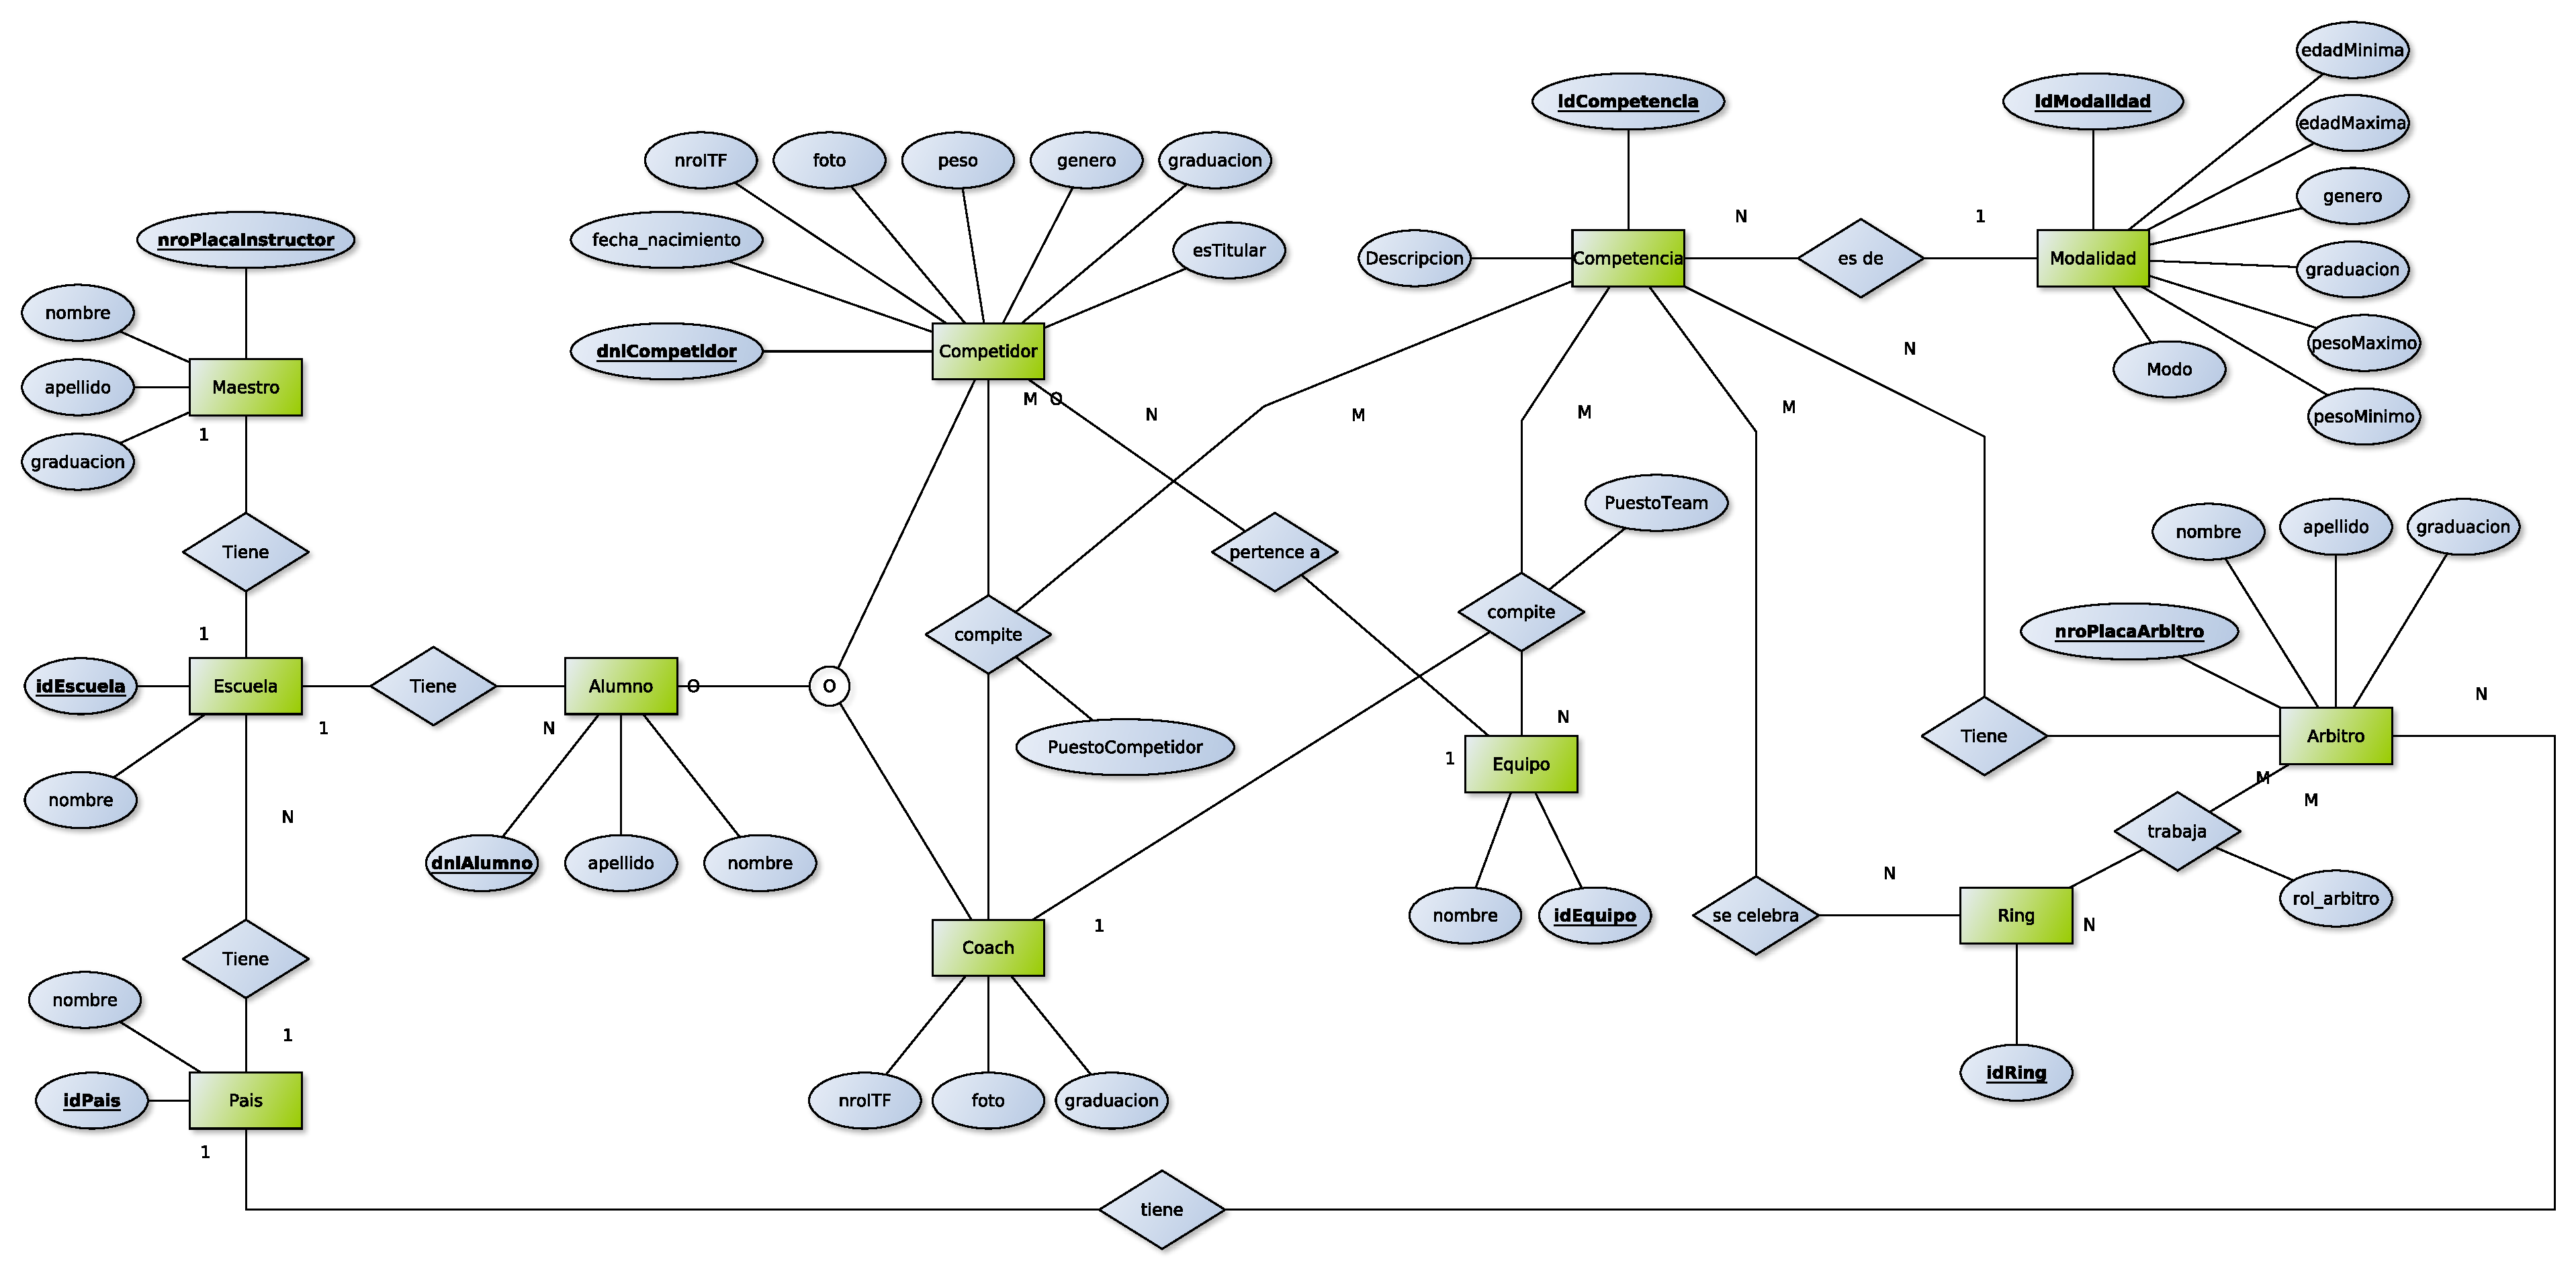
\includegraphics[width=20cm,keepaspectratio,angle=90]{./imagenes/DER.pdf}\newline
\end{center}

\newpage
\subsection{Modelo Relacional}

\noindent\textbf{Escuela}(\uline{idEscuela}, nombre, \dashuline{idPais}, \dashuline{nroPlacaInstructor}) 
\\
\\
PK = CK = \{ idEscuela \} \\
FK = \{ idPais, nroPlacaInstructor \} \\

\noindent\textbf{Pais}(\uline{idPais}, nombre)
\\
\\
PK = CK = \{ idPais \} \\

\noindent\textbf{Maestro}(\uline{nroPlacaInstructor}, nombre, apellido, graduación)
\\
\\
PK = CK = \{ nroPlacaInstructor \} \\

\noindent\textbf{Alumno}(\uline{dniAlumno}, nombre, apellido, \dashuline{idEscuela})
\\
\\
PK = CK = \{ dniAlumno \} \\
FK = \{ idEscuela \} \\

\noindent\textbf{Coach}(\uuline{dniAlumno}, nroITF, foto, graduación)
\\
\\
PK = CK = FK = \{ dniAlumno \} \\

\textit{Restricciones:}
\begin{itemize}
	\item Un alumno puede \textbf{no} estar en Coach
\end{itemize}

\noindent\textbf{Competidor}(\uline{dniCompetidor}, nroITF, fechaNacimiento, género, graduación, peso, foto, \dashuline{idEquipoTitular}, \dashuline{idEquipoSuplente})
\\
\\
PK = CK = \{ dniCompetidor \} \\
FK = \{ idEquipoTitular, idEquipoSuplente \} \\


\textit{Restricciones:}
\begin{itemize}
	\item Un alumno puede \textbf{no} estar en Competidor.
	\item El Competidor puede \textbf{no} estar en Equipo.
	\item Si el Competidor estar en Equipo, entonces es Titular ó es Suplente. No puede cumplir los dos roles en Equipo.
\end{itemize}


\noindent\textbf{senseiInscribeAlumno}(\uuline{dniCompetidor}, \uuline{dniAlumno}, \dashuline{nroPlacaInstructor})
\\
\\
PK = \{ (dniCompetidor,dniAlumno) \} \\
CK = \{ (dniCompetidor,dniAlumno), (dniCompetidor,nroPlacaInstructor), (dniAlumno,nroPlacaInstructor)\} \\
FK = \{ dniCompetidor, dniAlumno, nroPlacaInstructor \} \\


\noindent\textbf{Equipo}(\uline{idEquipo}, nombre)
\\
\\
PK = CK = \{ idEquipo \} \\


\noindent\textbf{Competencia}(\uline{idCompetencia}, descripcion, oro, plata, bronce, \dashuline{idModalidad})
\\
\\
PK = CK = \{ idCompetencia \} \\
FK = \{ idModalidad \} \\

\textit{Restricciones:}
\begin{itemize}
	\item Competencia guarda los dni de los ganadores. En Oro el dni del primer puesto de la competencia, en plata el dni del segundo puesto, y en bronce el dni del tercer puesto. (esta son FK DUDA)
\end{itemize}

\noindent\textbf{compiteEnCompetenciaInd}(\uuline{dniCompetidor}, \uuline{idCompetencia}, \dashuline{dniCoach})
\\
\\
PK = \{ (dniCompetidor,idCompetencia) \} \\
CK = \{ (dniCompetidor,idCompetencia), (dniCompetidor,dniCoach), (idCompetencia,dniCoach)\} \\
FK = \{ dniCompetidor, idCompetencia, dniCoach \} \\

\noindent\textbf{compiteEnCompetenciaTeam}(\uuline{idEquipo}, \uuline{idCompetencia}, \dashuline{dniCoach})
\\
\\
PK = \{ (idEquipo,idCompetencia) \} \\
CK = \{ (idEquipo,idCompetencia), (idEquipo,idCompetencia), (idCompetencia,dniCoach)\} \\
FK = \{ idEquipo, idCompetencia, dniCoach \} \\

\noindent\textbf{Modalidad}(\uline{idModalidad}, edad, género, graduación, peso, modo)
\\
\\
PK = CK = \{ idModalidad \} \\

\noindent\textbf{Ring}(\uline{idRing})
\\
\\
PK = CK = \{ idRing \} \\

\noindent\textbf{Arbitro}(\uline{nroPlacaArbitro}, nombre, apellido, graduación, \dashuline{idPais})
\\
\\
PK = CK = \{ nroPlacaArbitro \} \\
FK = \{ idPais \} \\

\noindent\textbf{arbitrosEnCompetencias}(\uuline{nroPlacaArbitro}, \uuline{idCompetencia})
\\
\\
PK = CK = FK = \{ (nroPlacaArbitro,idCompetencia) \} \\

\noindent\textbf{ringsDeCompetencias}(\uuline{idRing}, \uuline{idCompetencia})
\\
\\
PK = CK = FK = \{ (idRing,idCompetencia) \} \\

\noindent\textbf{puestoArbitroEnRing}(\uuline{nroPlacaArbitro},\uuline{idRing}, puesto)
\\
\\
PK = CK = FK = \{ (nroPlacaArbitro,idRing) \} \\
